\documentclass[12pt]{article}

\usepackage{sbc-template}
\usepackage{graphicx,url}
\usepackage[utf8]{inputenc}
\usepackage[brazilian]{babel}
\usepackage{amssymb}
\usepackage{booktabs}
\usepackage{multirow}
\usepackage{tikz}
\usetikzlibrary{positioning,babel}

% Linhas de tabela geradas (tab_*.tex) lidas pelo \input primitivo: no LaTeX
% recente (TeX Live 2026, Overleaf) o \input executa ganchos que quebram o
% \midrule ou \bottomrule logo após o arquivo.
\makeatletter
\newcommand{\tabinput}[1]{\@@input #1.tex }
\makeatother

\sloppy

\title{Análise do Impacto da Hierarquia de Memória em GPU AMD Utilizando OpenCL}

\author{Henrique de Almeida Diniz\inst{1}, Pedro Henrique Ramos Costa\inst{1}}

\address{Instituto de Ciências Exatas e de Informática\\
  Pontifícia Universidade Católica de Minas Gerais (PUC Minas)\\
  Belo Horizonte, MG -- Brasil
  \email{henriquealdiniz@gmail.com, phramoscosta@gmail.com}
}

\begin{document}

\maketitle

\begin{abstract}
This work analyses the impact of the memory hierarchy on the performance of an
AMD Ellesmere GPU (GCN, GFX8) under OpenCL, using as instrument the control of
cache flags through inline assembly verified in the ISA, since \texttt{volatile}
depends on the compiler. Across four experiments, the cost of bypassing the L1,
isolated by a controlled design, falls from 1.20$\times$ to 1.06$\times$ over a
256-fold range in data volume and ranges from 2.19$\times$ to 1.01$\times$ with
access locality; by the same mechanism, transposing a matrix, a classic CPU
optimization, makes multiplication 2.3--2.5$\times$ slower. For FLAT loads, SLC=1
does not bypass the L2: a working set that fits in it sustains 555.9~GB/s, above
the 256~GB/s theoretical peak of the VRAM.
\end{abstract}

\begin{resumo}
Este trabalho analisa o impacto da hierarquia de memória no desempenho de uma
GPU AMD Ellesmere (GCN, GFX8) sob OpenCL, usando como instrumento o controle das
\textit{flags} de \textit{cache} por \textit{inline assembly} verificado na ISA,
já que o \texttt{volatile} depende do compilador. Em quatro experimentos, o custo
de contornar o L1, isolado por desenho controlado, cai de 1,20$\times$ para
1,06$\times$ ao longo de um fator de 256 em volume de dados e vai de
2,19$\times$ a 1,01$\times$ conforme a localidade do acesso; pelo mesmo mecanismo,
transpor uma matriz, otimização clássica em CPU, torna a multiplicação 2,3 a
2,5$\times$ mais lenta. Em leituras FLAT, SLC=1 não contorna o L2: um conjunto que cabe nele
sustenta 555,9~GB/s, acima do pico teórico de 256~GB/s da VRAM.
\end{resumo}

\section{Introdução}

A computação paralela em unidades de processamento gráfico (GPUs) tornou-se uma estratégia consolidada para a aceleração de algoritmos que demandam alto poder computacional. \textit{Frameworks} como CUDA e OpenCL permitem que desenvolvedores utilizem os milhares de núcleos disponíveis nas GPUs modernas para executar tarefas de propósito geral, prática conhecida como GPGPU (\textit{General-Purpose computing on the GPU}) \cite{fang2011}. Nesse contexto, o OpenCL destaca-se por ser um padrão aberto e portável, capaz de executar código em dispositivos de diferentes fabricantes, incluindo GPUs AMD, NVIDIA e Intel, além de CPUs e outros aceleradores \cite{seo2011}.

Embora o paralelismo massivo oferecido pelas GPUs seja fundamental para o desempenho de algoritmos paralelos, a forma como os dados são acessados na memória exerce um impacto igualmente significativo. GPUs modernas possuem uma hierarquia de memória composta por múltiplos níveis: registradores, memória local (LDS), \textit{caches} L1 e L2 e memória global (VRAM), cada qual com características distintas de latência e largura de banda \cite{ariel2012}. Como os níveis mais próximos do processador são menores e mais rápidos, a eficiência de um algoritmo paralelo depende diretamente de quão bem ele explora essa hierarquia.

Diante desse cenário, a pergunta que orienta este trabalho é: qual é o impacto quantitativo da hierarquia de memória no desempenho de algoritmos paralelos executados em GPU AMD utilizando OpenCL? A literatura existente concentra-se predominantemente em GPUs NVIDIA \cite{ariel2012, fang2011, wong2010, jia2012, mei2017, jia2018}, havendo escassez de estudos que investiguem o comportamento de \textit{cache} e memória em GPUs AMD da arquitetura GCN sob OpenCL. Além disso, medir esse impacto exige retirar um nível do caminho de um acesso, e a interação entre o compilador OpenCL e a arquitetura no controle de \textit{cache} permanece pouco explorada.

A relevância é prática e metodológica. Saber quanto um nível de \textit{cache} vale, e do que esse valor depende, orienta decisões de otimização, como a disposição dos dados na memória; e medi-lo sem confundi-lo com efeitos de geração de código exige um instrumento verificado no binário, ausente da literatura sobre GPUs AMD sob OpenCL.

O objetivo geral deste trabalho é analisar experimentalmente o impacto da hierarquia de memória no desempenho de algoritmos paralelos executados em GPU AMD (arquitetura Polaris/GCN) sob OpenCL. Para isso, definem-se os objetivos específicos:

\begin{enumerate}
\item Obter e verificar, na ISA, um mecanismo que permita retirar o L1 do caminho de uma leitura a partir de código OpenCL no GFX8.
\item Isolar, por desenho controlado, o custo de contornar o L1, separando-o dos fatores que a comparação ingênua confunde com ele.
\item Determinar quais limites da hierarquia são efetivamente selecionáveis por \textit{flags} de instrução, testando a hipótese de que SLC=1 contorna o L2.
\item Verificar como o custo de contornar o L1 varia com o tamanho do problema e com a localidade do padrão de acesso, inclusive em um algoritmo completo.
\end{enumerate}

Em síntese, o instrumento foi obtido por \textit{inline assembly}, pois o \texttt{volatile} mostrou-se dependente do compilador, e empregado em quatro experimentos centrados na multiplicação de matrizes. O custo de contornar o L1 cai de 1,20$\times$ para 1,06$\times$ com o tamanho do problema e varia de 2,19$\times$ a 1,01$\times$ com a localidade, governado pelo reúso dentro da linha de \textit{cache}; transpor uma das matrizes, otimização clássica em CPU, torna a multiplicação 2,3 a 2,5$\times$ mais lenta; e, em leituras FLAT, SLC=1 não contorna o L2, de modo que apenas o L1 é selecionável por \textit{flags}.

O texto organiza-se assim: a Seção~2 apresenta o referencial teórico; a Seção~3 discute os trabalhos relacionados e posiciona a contribuição; a Seção~4 descreve a metodologia; a Seção~5, os resultados; e a Seção~6, as conclusões e os trabalhos futuros.

\section{Referencial Teórico}

\subsection{GPGPU e o Modelo de Memória do OpenCL}

Diferentemente das CPUs, projetadas para minimizar a latência de tarefas individuais, as GPUs maximizam o \textit{throughput} de operações simultâneas sobre centenas a milhares de núcleos~\cite{fang2011}, o que as torna adequadas a algoritmos de paralelismo de dados uniforme, como a multiplicação de matrizes. O desempenho ótimo, porém, costuma exigir otimizações específicas de plataforma~\cite{memeti2017, seo2011, vidye2023}.

O OpenCL organiza a execução em \textit{kernels}, instanciados como \textit{work-items} agrupados em \textit{work-groups} que executam numa mesma \textit{compute unit} (CU). Seu modelo de memória distingue quatro regiões (\textit{global}, \textit{constant}, \textit{local} e \textit{private}), cuja latência e largura de banda diferem em ordens de grandeza~\cite{fraire2013}. É a região \textit{global}, atendida pela VRAM através dos \textit{caches}, que este trabalho investiga: o modelo do OpenCL nomeia as regiões, mas não expõe qual nível de \textit{cache} atende cada acesso, e é precisamente esse controle que se busca aqui.

\subsection{Hierarquia de Memória em GPUs AMD (GCN/Polaris)}

As GPUs AMD baseadas na arquitetura GCN (\textit{Graphics Core Next}), como a família Polaris (RX 470/480/570/580, codinome Ellesmere), possuem uma hierarquia de memória composta por múltiplos níveis. Os registradores constituem a memória privada de cada \textit{work-item}, com latência mínima. O LDS (\textit{Local Data Share}) oferece 64~KB de memória compartilhada por CU, correspondendo à memória \texttt{\_\_local} do OpenCL. O \textit{cache} L1 (vL1), com 16~KB por CU e política \textit{write-through}, é utilizado para leituras de memória global. O \textit{cache} L2, compartilhado entre todas as CUs, possui capacidade de até 2~MB na Polaris e reside no mesmo \textit{die} da GPU, particionado entre os controladores de memória.\footnote{A consulta \texttt{CL\_DEVICE\_GLOBAL\_MEM\_CACHE\_SIZE} retorna 16~KB neste dispositivo, a capacidade do L1 por CU, não a do L2, que a API não expõe.} Por fim, a VRAM (memória global GDDR5) oferece alta largura de banda teórica (até 256~GB/s), porém com latência elevada em comparação aos \textit{caches} \cite{ariel2012}.

Na ISA GCN, as instruções de acesso à memória global (\texttt{buffer\_load\_dword} no formato MUBUF, \texttt{flat\_load\_dword} no formato FLAT) possuem campos de bits associados ao comportamento de \textit{cache}: GLC (\textit{Globally Coherent}) e SLC (\textit{System Level Coherent}). No formato FLAT do GFX8, o bit~16 corresponde a GLC e o bit~17 a SLC; no formato MUBUF, GLC ocupa o bit~14 e SLC o bit~17~\cite{amdgcn3}. A nomenclatura sugere que GLC controlaria a coerência no L1 e SLC no nível de sistema, e o próprio manual descreve o SLC de duas formas: nos formatos MUBUF e MTBUF, os acessos com SLC=1 são forçados a faltar no L2 e ficam coerentes com a memória do sistema; no FLAT, o bit define a política de \textit{cache} junto com GLC e com o tipo de memória (MTYPE)~\cite[Tabelas~8.2 e~9.1]{amdgcn3}. O efeito efetivo de cada bit no GFX8 é objeto de investigação neste trabalho, e a Seção~\ref{sec:slc} mostra que, em leituras FLAT, a primeira descrição não se aplica.

Mecanismos como o qualificador \texttt{volatile} e o \textit{inline assembly} GCN (\texttt{\_\_asm\_\_}) poderiam, em tese, controlar esses bits a partir de código OpenCL; o que cada um de fato produz no GFX8 é verificado na Seção~\ref{sec:multi}.

\section{Trabalhos Relacionados}

\subsection{Comparação de \textit{Frameworks} para GPGPU}

Um primeiro eixo da literatura compara \textit{frameworks} de programação paralela. Fang et al.~\cite{fang2011} avaliaram CUDA e OpenCL em 16 \textit{kernels} sobre GPUs NVIDIA e atribuíram parte da desvantagem do OpenCL a padrões de acesso à memória menos eficientes gerados pelo seu compilador; Memeti et al.~\cite{memeti2017} mediram variações de até uma ordem de grandeza entre implementações otimizadas e não otimizadas, conforme o \textit{framework} e as otimizações de memória; e Fraire et al.~\cite{fraire2013} ressaltaram o peso do modelo de memória e da organização dos \textit{work-items}. Seo et al.~\cite{seo2011}, ao portarem os \textit{NAS Parallel Benchmarks} para OpenCL, mostraram que a eficiência do acesso à memória frequentemente supera o paralelismo computacional como determinante do desempenho. O conjunto estabelece a premissa deste trabalho, a de que o acesso à memória domina, e localiza no \textbf{compilador} uma fonte de variação que a Seção~\ref{sec:multi} retoma de forma direta.

\subsection{Hierarquia de Memória em GPUs}

No contexto específico da hierarquia de memória, Wong et al.~\cite{wong2010} propuseram uma metodologia de microbenchmarking baseada em \textit{pointer chasing} (P-chase) para mapear experimentalmente os tamanhos e latências dos \textit{caches} de GPUs NVIDIA (GeForce GTX 280, arquitetura GT200). A técnica consiste em percorrer uma lista encadeada cujo tamanho determina o \textit{working set}: quando o conjunto de trabalho cabe no \textit{cache} L1, a latência medida é baixa; ao ultrapassar esse limiar, a latência aumenta abruptamente, revelando a capacidade de cada nível. Essa metodologia orienta a caracterização dos níveis de \textit{cache} que fundamenta este trabalho, embora o desenho aqui adotado meça vazão sob carga, e não latência isolada.

Mei e Chu~\cite{mei2017} refinaram a técnica e a aplicaram de Fermi a Pascal, demonstrando que a latência apresenta ``degraus'' característicos nas transições entre níveis, o que permite mapear com precisão a capacidade de cada um.

Jia et al.~\cite{jia2018} estenderam a abordagem à arquitetura Volta, combinando microbenchmarks com desassemblagem de instruções para caracterizar a geometria e as latências de cada nível. Como em Wong et al. e Mei e Chu, os experimentos foram conduzidos exclusivamente em GPUs NVIDIA com CUDA, o que evidencia a lacuna para arquiteturas AMD. A combinação de microbenchmarking com análise de ISA é o método aqui adaptado para GPUs AMD sob OpenCL.

Mais próximos desta pergunta, Jia, Shaw e Martonosi~\cite{jia2012} ligaram e desligaram o L1 de uma GPU Fermi: ele acelerou alguns programas e retardou outros, e o tráfego L1--L2 previu o efeito melhor que a taxa de acerto. Daí derivaram uma taxonomia de localidade (dentro do \textit{warp}, entre \textit{warps} e entre instruções) que decide o uso do L1 por \textit{load}.

Em GPUs AMD a caracterização é bem mais escassa. Tee e Wong~\cite{tee2025} aplicaram microbenchmarking de latência à CDNA~3, mapeando o comportamento dos \textit{caches} compartilhados e do \textit{Infinity Cache}. O trabalho confirma que a técnica se transporta para GPUs AMD, mas incide sobre uma arquitetura de centro de dados muito posterior à GCN e não trata dos mecanismos de programação que selecionam o nível de \textit{cache}, objeto deste estudo.

Bernal et al.~\cite{ariel2012} propuseram um modelo estocástico para a hierarquia de memória de GPUs, capaz de estimar taxas de \textit{hit/miss} e latências efetivas.

\subsection{Influência da Plataforma e do Sistema Operacional}

Vidye et al.~\cite{vidye2023} avaliaram o OpenCL em Windows, Linux e macOS, identificando variações significativas no tempo de execução conforme a plataforma: o mesmo código pode se comportar de modo distinto segundo o SO e o \textit{driver}, o que reforça a relevância de estudos por plataforma.

Balen et al.~\cite{balen2022} avaliaram o desempenho de diferentes distribuições Linux em tarefas computacionais, demonstrando que a configuração do sistema operacional afeta significativamente o desempenho de aplicações.

Ambos atribuem ao sistema operacional as diferenças entre plataformas, e o resultado deste estudo qualifica essa atribuição: a diferença observada entre dois ambientes sobre o mesmo dispositivo não decorre do SO, mas do \textit{front-end} do compilador de \textit{kernels} de cada um (Seção~\ref{sec:metodologia-ambiente}). Comparações que não isolem o compilador arriscam imputar ao ambiente um efeito de geração de código.

\subsection{Síntese e Posicionamento}

\begin{table}[ht]
\centering
\caption{Comparação dos trabalhos relacionados.}
\label{tab:trabalhos}
\resizebox{\textwidth}{!}{%
\begin{tabular}{@{}lccccl@{}}
\toprule
\textbf{Trabalho} & \textbf{GPU} & \textbf{Framework} & \textbf{SO} & \textbf{Hier. Mem.} & \textbf{Foco principal} \\
\midrule
Fang et al. (2011) & NVIDIA & CUDA/OpenCL & Linux & Não & Comparação de \textit{frameworks} \\
Seo et al. (2011) & NVIDIA & OpenCL & Linux & Parcial & Caracterização de \textit{benchmarks} \\
Wong et al. (2010) & NVIDIA & CUDA & Linux & Sim & Microbenchmarking de \textit{cache} \\
Mei e Chu (2017) & NVIDIA & CUDA & Linux & Sim & Latência por nível de \textit{cache} \\
Jia et al. (2018) & NVIDIA & CUDA & Linux & Sim & Microarquitetura Volta \\
Jia, Shaw e Martonosi (2012) & NVIDIA & CUDA & --- & Sim & Valor do L1 e localidade \\
Bernal et al. (2012) & NVIDIA & CUDA & Linux & Sim & Modelo estocástico de \textit{cache} \\
Memeti et al. (2017) & NVIDIA & Múltiplos & Linux & Parcial & Produtividade e desempenho \\
Fraire et al. (2013) & NVIDIA & OpenCL & --- & Parcial & Comparação CPU vs GPU \\
Vidye et al. (2023) & Múltiplas & OpenCL & Múltiplos & Não & Portabilidade entre SOs \\
Balen et al. (2022) & --- & --- & Linux & Não & Desempenho de SOs \\
Tee e Wong (2025) & AMD & ROCm & Linux & Sim & \textit{Caches} compartilhados (CDNA~3) \\
\midrule
\textbf{Este trabalho} & \textbf{AMD} & \textbf{OpenCL} & \textbf{Win/Linux} & \textbf{Sim} & \textbf{Hierarquia de memória GCN} \\
\bottomrule
\end{tabular}%
}
\end{table}

Conforme a Tabela~\ref{tab:trabalhos}, a literatura concentra-se em GPUs NVIDIA sob Linux. Este estudo investiga uma GPU AMD GCN/Polaris sob OpenCL e desloca o objeto de análise: onde o microbenchmarking caracteriza a \emph{geometria} da hierarquia (capacidade e latência de cada nível), aqui se mede quanto um nível vale, como Jia, Shaw e Martonosi~\cite{jia2012} no Fermi. Lá o controle é oferecido pelo CUDA; aqui precisa ser construído e verificado na ISA, e seu custo, separado do efeito do \textit{cache}.

\section{Metodologia}
\label{sec:metodologia-ambiente}

Os experimentos são conduzidos em uma GPU AMD Ellesmere (RX 580 8~GB, arquitetura
GCN 4\textordfeminine{} geração, GFX8) com 36 \textit{Compute Units} a 1350~MHz,
\textit{cache} L1 de 16~KB por CU (\textit{write-through}), \textit{cache} L2 de
2~MB compartilhado, LDS de 64~KB por CU e 8~GB de VRAM GDDR5. O ambiente de
software é Ubuntu com \textit{kernel} 5.15 e ROCm~5.2, cujo compilador de
\textit{kernel} é o Clang/LLVM embutido no \texttt{comgr}; a arquitetura Polaris é
depreciada nessa versão, e o dispositivo só é enumerado com a variável de ambiente
\texttt{ROC\_ENABLE\_PRE\_VEGA=1}. O anfitrião é compilado com GCC e a ISA é
desmontada com \texttt{llvm-objdump}. A metodologia compreende a obtenção do
instrumento de medição e quatro experimentos, esquematizados na
Figura~\ref{fig:hierarquia}.

A escolha do ambiente decorre de etapa anterior deste trabalho, conduzida sobre o
mesmo dispositivo físico em Windows, cujo compilador proprietário do
\textit{driver} (AMDOCL) não aceita \textit{inline assembly} nem emite
\textit{flags} sob \texttt{volatile} (Seção~\ref{sec:multi}).

O desenho parte de três caminhos candidatos para uma mesma leitura (atendida
pelo L1; pelo L2, com desvio do L1; e pela memória global, com desvio de ambos),
que é o que a nomenclatura das \textit{flags} GLC e SLC sugere. Quais deles são de
fato obteníveis no GFX8 não é premissa, mas objeto de verificação: o
Experimento~2 submete o terceiro a teste (Seção~\ref{sec:slc}). Adiante-se que,
em leituras FLAT, apenas os dois primeiros existem, de modo que os experimentos comparam
\textbf{dois caminhos de memória}, e não três.

\begin{figure}[ht]
\centering
% Diagrama da Metodologia: caminhos de uma leitura na hierarquia do gfx803 e
% o que cada experimento mede. Incluído em main.tex por % Diagrama da Metodologia: caminhos de uma leitura na hierarquia do gfx803 e
% o que cada experimento mede. Incluído em main.tex por % Diagrama da Metodologia: caminhos de uma leitura na hierarquia do gfx803 e
% o que cada experimento mede. Incluído em main.tex por \input{fig_hierarquia}.
\begin{tikzpicture}[
  font=\footnotesize,
  nivel/.style={draw, rounded corners=2pt, minimum height=0.9cm,
                minimum width=2.3cm, align=center, fill=black!5},
  seta/.style={-latex, semithick},
  node distance=1.25cm,
]
\node[nivel] (wi) {\textit{Work-item}\\registradores};
\node[nivel, right=of wi] (l1) {L1 vetorial\\16~KB por CU};
\node[nivel, right=of l1] (l2) {L2\\2~MB};
\node[nivel, right=of l2] (vr) {VRAM\\GDDR5, 8~GB};
\draw[seta] (wi) -- node[above=1pt, font=\scriptsize]{\texttt{GLC=0}} (l1);
\draw[seta] (l1) -- (l2);
\draw[seta] (l2) -- (vr);
\draw[seta] (wi.north) to[out=20, in=160]
  node[above=-1pt]{\texttt{glc}: contorna o L1 (Exp.~1, 3 e 4)} (l2.north);
\draw[seta, dashed] (wi.south) to[out=-14, in=-166]
  node[below=-1pt]{\texttt{slc}: acesso direto à VRAM? (Exp.~2)}
  (vr.south);
\end{tikzpicture}
.
\begin{tikzpicture}[
  font=\footnotesize,
  nivel/.style={draw, rounded corners=2pt, minimum height=0.9cm,
                minimum width=2.3cm, align=center, fill=black!5},
  seta/.style={-latex, semithick},
  node distance=1.25cm,
]
\node[nivel] (wi) {\textit{Work-item}\\registradores};
\node[nivel, right=of wi] (l1) {L1 vetorial\\16~KB por CU};
\node[nivel, right=of l1] (l2) {L2\\2~MB};
\node[nivel, right=of l2] (vr) {VRAM\\GDDR5, 8~GB};
\draw[seta] (wi) -- node[above=1pt, font=\scriptsize]{\texttt{GLC=0}} (l1);
\draw[seta] (l1) -- (l2);
\draw[seta] (l2) -- (vr);
\draw[seta] (wi.north) to[out=20, in=160]
  node[above=-1pt]{\texttt{glc}: contorna o L1 (Exp.~1, 3 e 4)} (l2.north);
\draw[seta, dashed] (wi.south) to[out=-14, in=-166]
  node[below=-1pt]{\texttt{slc}: acesso direto à VRAM? (Exp.~2)}
  (vr.south);
\end{tikzpicture}
.
\begin{tikzpicture}[
  font=\footnotesize,
  nivel/.style={draw, rounded corners=2pt, minimum height=0.9cm,
                minimum width=2.3cm, align=center, fill=black!5},
  seta/.style={-latex, semithick},
  node distance=1.25cm,
]
\node[nivel] (wi) {\textit{Work-item}\\registradores};
\node[nivel, right=of wi] (l1) {L1 vetorial\\16~KB por CU};
\node[nivel, right=of l1] (l2) {L2\\2~MB};
\node[nivel, right=of l2] (vr) {VRAM\\GDDR5, 8~GB};
\draw[seta] (wi) -- node[above=1pt, font=\scriptsize]{\texttt{GLC=0}} (l1);
\draw[seta] (l1) -- (l2);
\draw[seta] (l2) -- (vr);
\draw[seta] (wi.north) to[out=20, in=160]
  node[above=-1pt]{\texttt{glc}: contorna o L1 (Exp.~1, 3 e 4)} (l2.north);
\draw[seta, dashed] (wi.south) to[out=-14, in=-166]
  node[below=-1pt]{\texttt{slc}: acesso direto à VRAM? (Exp.~2)}
  (vr.south);
\end{tikzpicture}

\caption{Caminhos de uma leitura na hierarquia do gfx803. O instrumento
(Seção~\ref{sec:multi}) seleciona o caminho pelas \textit{flags} da instrução de
\textit{load}; os Experimentos~3 e~4 medem o custo de contornar o L1 em função do
tamanho do problema e do padrão de acesso.}
\label{fig:hierarquia}
\end{figure}

\subsection{Obtenção e Verificação do Instrumento}
\label{sec:met-multi}
\label{sec:multi}

Cada mecanismo candidato é avaliado por um único critério: a instrução
efetivamente emitida, extraída por \texttt{clGetProgramInfo(CL\_PROGRAM\_BINARIES)}
e desmontada para \texttt{mcpu=gfx803}, sobre \textit{kernels} de multiplicação de
matrizes $1024 \times 1024$ verificados contra referência em CPU. O
\texttt{volatile} não serve como instrumento por duas razões. A emissão da
\textit{flag} depende do compilador: o Clang/LLVM troca \texttt{DC500000} (GLC=0)
por \texttt{DC510000} (GLC=1), e o compilador proprietário mantém GLC=0. E, mesmo
sob o Clang, o \textit{codegen} insere \texttt{s\_waitcnt vmcnt(0)} após cada
\textit{load}, serializando acessos independentes, de modo que seu tempo não mede
apenas o desvio do \textit{cache}. O atributo \texttt{address\_space(1)} não emite
\textit{flag} alguma, pois no AMDGPU o espaço~1 é o próprio espaço global.

Adotou-se o \textit{inline assembly} GCN no formato FLAT
(\texttt{flat\_load\_dword}), que aceita os modificadores \texttt{glc} e
\texttt{slc} e produz as quatro combinações com os bits nas posições esperadas
(\texttt{DC500000}, \texttt{DC510000}, \texttt{DC520000} e \texttt{DC530000}). O
formato MUBUF é viável, mas exige um descritor de recurso de 128 bits cuja má
formação devolve leituras silenciosamente nulas; o \textit{builtin}
\texttt{\_\_builtin\_nontemporal\_load} emite \texttt{glc slc} sem
\textit{assembly}, mas não permite \texttt{glc} isolado. Nenhuma instrução de
escrita recebe \texttt{glc} (as escritas alcançam o L2 porque o L1 do GCN é
\textit{write-through}), razão pela qual o trabalho investiga apenas leituras.

\subsection{Experimento 1: Isolamento do Efeito do L1}
\label{sec:met-fatorial}

A comparação direta entre o \textit{kernel} normal e um com \textit{bypass} não permite atribuir a diferença ao \textit{cache}, porque dois outros fatores variam junto com a \textit{flag}: o \textit{codegen} do \texttt{volatile}, que serializa os \textit{loads} (Seção~\ref{sec:multi}); e o próprio bloco de \textit{inline assembly}, opaco ao otimizador, que impede a redução de força no cálculo de endereço~\cite{granlund1994} e acrescenta ALU por iteração.

Para separá-los, o experimento emprega seis \textit{kernels} com o mesmo algoritmo e \textit{work-groups} de $16\times16$, variando apenas o caminho de memória, entre eles um \textbf{controle} construído em \textit{assembly} sem \textit{flag} alguma, que reproduz a construção das variantes com \textit{flag} sem alterar o caminho de memória.

Cada cenário é executado 1000 vezes após 10 de aquecimento, registrando-se média, mediana, desvio padrão, coeficiente de variação e a deriva entre o primeiro e o último décimo das execuções, esta para detectar variação de \textit{clock} sob carga sustentada. As razões vêm acompanhadas de intervalo de confiança de 95\% pelo método delta. Como com $n=1000$ o teste de significância passa a acusar até a diferença entre dois \textit{kernels} de ISA idêntica, adota-se um \textbf{piso de ruído} dado pela diferença medida entre um par de \textit{kernels} de fonte idêntico; efeitos menores não são afirmados. Todos são verificados elemento a elemento contra a CPU, e o experimento é repetido em $N=1024$ e $N=1008$.

\subsection{Experimento 2: Semântica do Bit SLC}
\label{sec:met-slc}

Para decidir se \texttt{SLC=1} realiza o \textit{bypass} do L2, mede-se a vazão da leitura repetida de um mesmo \textit{buffer} em função do seu tamanho. As três variantes (sem \textit{flags}, \texttt{glc} e \texttt{glc slc}) são construídas por \textit{inline assembly} com \texttt{flat\_load\_dword} sobre \textit{buffers} comuns, alocados na VRAM, de modo que a geração de código é idêntica e a única diferença são os bits da instrução. Cada lançamento percorre o \textit{buffer} ciclicamente e lê 128~MiB, relendo 128 vezes um \textit{buffer} de 1~MB, que \textbf{cabe} no L2 de 2~MB, e duas vezes um de 64~MB, que \textbf{não cabe}; acima de 64~MB, lê o \textit{buffer} duas vezes. A campanha original mediu esses dois tamanhos; uma segunda campanha repete os mesmos \textit{kernels} em 14 tamanhos, de 256~KB a 2~GB, e lê cada \textit{buffer} por 0,2~s antes de medir, para estabilizar os \textit{clocks}.

O teste depende de saber quanto a VRAM entregaria se o L2 fosse contornado. Além do pico teórico da GDDR5, nove variantes com 4 a 16 vezes mais bytes em voo por \textit{wavefront} (cargas de 16~B, várias cargas antes da espera e diferentes números de \textit{work-items}) leem um \textit{buffer} de 1~GB, para separar o limite da memória do limite do \textit{kernel} de medição. Dois controles verificam o caso de 1~MB: como, no programa original, \texttt{glc slc} roda depois de dois \textit{kernels} que deixam o \textit{buffer} no L2, a leitura de outro \textit{buffer} de 64~MB, fora do tempo medido, ocupa o L2 antes de cada execução, em cinco tamanhos; e o caso de 1~MB é repetido em dez \textit{buffers} distintos.

\subsection{Experimento 3: Análise de Sensibilidade ao Tamanho do Problema}
\label{sec:met-sens}

Os Experimentos~1 e~2 medem os fatores em um único tamanho de problema. Nada
garante, porém, que o custo de contornar um nível de \textit{cache} seja
constante em relação ao tamanho: conforme o conjunto de trabalho cresce, muda a
fração dos acessos que o \textit{cache} conseguia atender, e com ela o que se
perde ao contorná-lo. Este experimento repete os cinco cenários em cinco tamanhos,
de $N=1024$ a $N=16384$, o que corresponde a um fator de 256 em volume de
dados, com 100 execuções medidas por ponto.

Como referência de escala, o mesmo algoritmo é medido na CPU do anfitrião (um
Intel Core Ultra~5 245KF, 14 \textit{threads}, 16~GB de DDR5), com paralelismo
de laço por OpenMP e nos mesmos cinco tamanhos. Usam-se todas as
\textit{threads}, pois medir um único núcleo contra 36 \textit{Compute Units}
inflaria a diferença por um fator que nada diz sobre os dispositivos; e mantém-se
o laço triplo ingênuo, de modo que a comparação isole o \textbf{dispositivo} com
a implementação constante. O número de execuções segue um orçamento de tempo por
tamanho, pois uma execução em $N=16384$ leva 3,3~h.

O limite superior é imposto pela memória: em $N=16384$ as três matrizes ocupam
3~GB dos 8~GB de VRAM disponíveis, e o tamanho seguinte da progressão excederia
tanto a VRAM quanto a memória de sistema.

Duas adaptações foram necessárias para tornar a análise exequível. A primeira
é a \textbf{referência amostrada}: como a verificação completa em CPU é $O(N^3)$
e em $N=16384$ custaria mais que a própria medição, a validação passa a ser feita
em duas camadas: cada cenário é comparado elemento a elemento com a saída do
cenário~1, em $O(N^2)$, e o cenário~1 é conferido contra referência de CPU sobre
uma amostra aleatória de 4.096 posições. A amostragem basta porque as falhas em
questão não são pontuais: um descritor mal formado devolve zero em todas as
posições, e uma \textit{flag} mal emitida altera o caminho de memória de todos
os acessos.

A segunda é o \textbf{lançamento em lotes} em $N=16384$, adotado por precaução,
já que a GPU também atende a saída de vídeo e um travamento derrubaria a sessão:
a \textit{NDRange} é fatiada por \texttt{global\_work\_offset} em faixas de 2.048
linhas, oito lançamentos por execução. O trabalho total
permanece idêntico e os \textit{kernels} não requerem alteração; verificou-se em
$N=2048$ que o modo em lotes produz resultado idêntico ao lançamento único, com
custo acrescido de 0,02~ms por lote.

\subsection{Experimento 4: Localidade do Padrão de Acesso}
\label{sec:met-localidade}

Os experimentos anteriores variam a \textit{flag} mantendo o padrão de acesso
fixo. Este inverte: mantém o controle de \textit{cache} e varia a localidade, para
responder quanto do valor do L1 depende do padrão que o exercita.

Os três padrões saem da própria multiplicação de matrizes, onde convivem, e leem
a \textbf{mesma matriz} com o \textbf{mesmo número de \textit{loads}}, $N$ por
\textit{work-item}, $N^3$ no total. Variam apenas nos índices; com
\textit{work-groups} de $16\times16$, cada \textit{wavefront} reúne 4 valores de
$\mathrm{row}$ e 16 de $\mathrm{col}$:

\begin{itemize}
\item \textbf{linha}, $A[\,\mathrm{row}\,N + k\,]$: $k$ avança 4~bytes, de modo que
16 acessos consecutivos caem na mesma linha de \textit{cache}; numa
\textit{wavefront} há 4 endereços, cada um pedido por 16 \textit{lanes}
(\textit{broadcast}).
\item \textbf{coluna}, $A[\,k\,N + \mathrm{col}\,]$: $k$ avança $4N$~bytes e cada
iteração toca uma linha nova; os \textit{lanes} pedem 16 endereços consecutivos,
numa única linha (coalescido).
\item \textbf{dispersa}, $A[\,((\mathrm{row}+\mathrm{col}) \bmod N)\,N + k\,]$:
passo contíguo como em \textbf{linha}, mas $\mathrm{row}+\mathrm{col}$ assume 19
valores na \textit{wavefront}, cada um pedido por até 4 \textit{lanes}.
\end{itemize}

O terceiro padrão existe porque \textbf{linha} e \textbf{coluna} diferem em dois
fatores, o passo em $k$ e o comportamento entre \textit{lanes};
comparar \textbf{linha} com \textbf{dispersa} troca só o segundo.

Cada padrão é medido nas três configurações de \textit{flag}, todas construídas
por \textit{inline assembly}, de modo que a razão entre elas não carregue custo de
construção. A validação é $O(N^2)$: a saída do padrão \textbf{linha} é a soma da
linha, a do \textbf{coluna} é a soma da coluna e a do \textbf{dispersa} é a soma da
linha deslocada, e bastam $N$ somas para conferir as $N^2$ posições. Cada medição é
um lançamento único da \textit{NDRange} inteira, sem fatiamento; após um
aquecimento, as execuções seguem um orçamento de 4~s por ponto (5 a 200).

Por fim, a multiplicação completa é executada com $B$ no \textit{layout} usual
($B[\,k\,N+\mathrm{col}\,]$, padrão \textbf{coluna}) e transposta no anfitrião,
otimização clássica em CPU ($B^{T}[\,\mathrm{col}\,N+k\,]$, padrão \textbf{dispersa}),
com $A$ no padrão \textbf{linha}, a construção do Experimento~1,
validação em 4.096 posições amostradas, lançamentos fatiados a partir de
$N=4096$ e orçamento de 6~s por ponto (5 a 100 execuções).

\section{Resultados}

\subsection{Experimento 1: Isolamento do Efeito do L1}
\label{sec:fatorial}

A Tabela~\ref{tab:cenarios} apresenta os cinco cenários para $N=1024$, com 1000 execuções cada. Todos foram verificados elemento a elemento contra a CPU, sem divergência, e a deriva ficou abaixo de 2\% em todos, o que afasta variação de \textit{clock} como explicação das diferenças.

\begin{table}[ht]
\centering
\caption{Cenários de caminho de \textit{cache}, $N=1024$; 1000 execuções por cenário de GPU e 25 na CPU. Tempos em ms; cv: desvio padrão sobre a média.}
\label{tab:cenarios}
\small
\begin{tabular}{@{}llrrrr@{}}
\toprule
\textbf{Cenário} & \textbf{\textit{Flags}} & \textbf{Média} & \textbf{Mediana} & \textbf{cv (\%)} & \textbf{GFLOPS} \\
\midrule
\multicolumn{6}{@{}l}{\textit{CPU (14 threads)}}\\
\quad laço triplo & --- & 247,3 & 247,3 & 3,87 & 8,7 \\
\midrule
\multicolumn{6}{@{}l}{\textit{GPU: cenários de caminho de \textit{cache}}}\\
1. Normal (OpenCL C) & GLC=0 SLC=0 & 7,265 & 7,223 & 3,50 & 297,3 \\
2. Controle: \textit{asm} sem \textit{flag} & GLC=0 SLC=0 & 10,985 & 11,007 & 1,86 & 195,1 \\
3. \texttt{volatile} & GLC=1 SLC=0 & 14,258 & 14,239 & 4,02 & 150,8 \\
4. \textit{asm} com \texttt{glc} & GLC=1 SLC=0 & 13,591 & 13,585 & 4,43 & 158,1 \\
5. \textit{asm} com \texttt{glc slc} & GLC=1 SLC=1 & 13,850 & 13,847 & 4,30 & 155,1 \\
\bottomrule
\end{tabular}
\end{table}

A referência em CPU situa a escala: com o mesmo algoritmo e as 14
\textit{threads} do anfitrião, ela leva 247,3~ms contra 7,223~ms do cenário~1;
a GPU é \textbf{34 vezes mais rápida}, por largura de paralelismo e não por o
\textit{hardware} da CPU ser mais lento. A Seção~\ref{sec:sens} mostra que essa
razão está longe de ser constante. Os demais cenários são todos \textit{kernels}
da mesma GPU.

O cenário~3 foi medido em duplicata, a partir de fonte idêntico e gerando ISA idêntica instrução a instrução; a réplica não é tabulada por ser redundante. O \textbf{controle negativo passa}: as duas medições diferem em 0,14\% e são estatisticamente indistinguíveis ($t=0{,}76$), o que valida a bancada. Essa diferença residual fixa o \textbf{piso de ruído} abaixo do qual nenhum efeito é afirmado; o piso é necessário porque, com $n=1000$, o erro padrão cai a ponto de o teste de significância acusar diferenças sem consequência prática.

A Tabela~\ref{tab:razoes} decompõe os fatores. O desenho se apoia no cenário~2, construído em \textit{assembly} sem \textit{flag} alguma: ele reproduz a mesma barreira de otimização dos cenários~4 e~5 sem alterar o caminho de memória, de modo que a comparação 2~$\to$~4 mede o bit \texttt{glc} com o custo da construção descontado dos dois lados. As três variantes em \textit{assembly} geram ISA idêntica instrução a instrução, diferindo apenas pelos modificadores \texttt{glc} e \texttt{slc} em dois \texttt{flat\_load\_dword}.

\begin{table}[ht]
\centering
\caption{Decomposição dos fatores. Razões entre médias, com intervalo de confiança de 95\% pelo método delta.}
\label{tab:razoes}
\small
\begin{tabular}{@{}llrl@{}}
\toprule
\textbf{Comparação} & \textbf{Fator isolado} & \textbf{Razão} & \textbf{IC 95\%} \\
\midrule
3 vs réplica & Piso de ruído (ISA idêntica) & 1,001$\times$ & [0,998; 1,005] \\
1 $\to$ 2 & Custo da construção em \textit{assembly} & 1,512$\times$ & [1,508; 1,516] \\
2 $\to$ 4 & \textit{Flag} \texttt{glc}, construção controlada & 1,237$\times$ & [1,234; 1,241] \\
4 $\to$ 5 & \textit{Flag} \texttt{slc} & 1,019$\times$ & [1,015; 1,023] \\
3 vs 4 & \texttt{volatile} contra \textit{asm} com \texttt{glc} & 1,049$\times$ & [1,045; 1,053] \\
\bottomrule
\end{tabular}
\end{table}

Três leituras decorrem da tabela. A primeira é que \textbf{a construção em \textit{assembly} responde sozinha por 1,512$\times$}, sem alterar o caminho de memória: sem o cenário de controle, esse custo seria atribuído ao \textit{cache}.

A segunda é que \textbf{o valor medido para a mesma \textit{flag} depende da linha de base contra a qual se mede}. Comparado diretamente ao cenário normal, o cenário~4 aparenta custar 1,871$\times$; com a construção em \textit{assembly} constante nos dois lados, \texttt{glc} custa 1,237$\times$. Não há contradição: o produto das duas razões, $1{,}512 \times 1{,}237 = 1{,}871$, reproduz a razão direta. A diferença entre elas é o custo de construção que a comparação ingênua atribuiria ao \textit{cache}. As duas respondem a perguntas distintas: quanto custa perder o L1 em código escrito dessa forma, e qual o efeito do bit isolado de todo o resto.

A terceira é a convergência entre mecanismos independentes: o \texttt{volatile} do ROCm e o \textit{inline assembly} com \texttt{glc} produzem tempos a 4,9\% um do outro. Já o efeito do \texttt{slc}, de 1,019$\times$, supera o piso de ruído de 0,14\% ($t=9{,}64$), mas é pequeno neste tamanho: os Experimentos~2 e~3 mostram que ele depende de haver pressão sobre o L2, o que em $N=1024$ ainda não há.

A repetição em $N=1008$ mostra que os fatores não são igualmente estáveis: o custo da construção em \textit{assembly} praticamente não varia (1,528$\times$ contra 1,512$\times$), enquanto o custo de contornar o L1 responde ao alinhamento: o \textit{stride} entre linhas de $B$ vale $4N$ bytes, e o número de fatores 2 desse valor determina quantos acessos colidem no mesmo conjunto do \textit{cache}, 12 em $N=1024$ contra 6 em $N=1008$.

\subsection{Experimento 2: Semântica do Bit SLC}
\label{sec:slc}

A Tabela~\ref{tab:slc} apresenta a leitura repetida nas duas campanhas: a
original, com \textit{buffers} de 1~MB e 64~MB, e a varredura de 256~KB a 2~GB.

\begin{table}[ht]
\centering
\caption{Leitura repetida por tamanho do \textit{buffer}; medianas de 25
execuções. Cada lançamento lê 128~MiB (duas passadas do \textit{buffer} acima de
64~MB); o L2 tem 2~MB, e o pico teórico da GDDR5 é de 256~GB/s. Razão: vazão de
\texttt{glc slc} sobre a de \texttt{glc}.}
\label{tab:slc}
\small
\setlength{\tabcolsep}{4pt}
\begin{tabular}{@{}llrrrrrrr@{}}
\toprule
 & & \multicolumn{3}{c}{\textbf{Tempo (ms)}} & \multicolumn{3}{c}{\textbf{Vazão (GB/s)}} & \\
\cmidrule(lr){3-5}\cmidrule(lr){6-8}
\textbf{\textit{Buffer}} & \textbf{L2} & sem \textit{flag} & \texttt{glc} & \texttt{glc slc} &
sem \textit{flag} & \texttt{glc} & \texttt{glc slc} & \textbf{Razão} \\
\midrule
\multicolumn{9}{@{}l}{\textit{Campanha original}}\\
\tabinput{tab_slc_original}
\midrule
\multicolumn{9}{@{}l}{\textit{Varredura (segunda campanha)}}\\
\tabinput{tab_slc}
\bottomrule
\end{tabular}
\end{table}

\textbf{O que um \textit{bypass} produziria.} Se \texttt{SLC=1} tirasse o L2 do
caminho, o \textit{buffer} de 1~MB passaria a ser lido da VRAM, e a vazão ficaria
sujeita a dois limites. O primeiro é físico: o pico teórico da GDDR5 desta placa,
256~GB/s (2.000~MHz em barramento de 256~bits), que nenhuma leitura atendida pela
VRAM ultrapassa, com ou sem \textit{bypass}. O segundo é o patamar que o mesmo
\textit{kernel} atinge quando o conjunto não cabe no L2: de 8~MB a 2~GB, sem
\textit{flag} e \texttt{glc} ficam entre 222,3 e 223,9~GB/s, cerca de 87\% do pico,
qualquer que seja o tamanho; os 222,3~GB/s de 64~MB da campanha original não
foram uma escolha de sorte. Esse patamar é da memória, e não do \textit{kernel}:
nenhuma das nove variantes com mais bytes em voo passa de 223,3~GB/s na mediana
(225,3 na melhor execução), e algumas caem a 196,3. Um \textit{bypass} limitaria,
portanto, o \textit{buffer} de 1~MB a no máximo 256~GB/s e, na prática, a cerca de
222~GB/s.

\textbf{O que se mede.} Em 1~MB, \texttt{glc slc} sustenta \textbf{555,9~GB/s} na
campanha original e 539,8~GB/s na varredura: 2,2 e 2,1 vezes o pico teórico, e
2,5 e 2,4 vezes o patamar medido na respectiva campanha. \textbf{A hipótese é
refutada}: o L2 continua atendendo os acessos. O valor de 1~MB varia com a
alocação: somadas todas as suas medições com \texttt{glc slc} (a da campanha
original, três reexecuções do programa original e 13 na segunda campanha, dez
delas em \textit{buffers} distintos), são 17 valores entre 431,5 e 564,1~GB/s
(mediana de 548,6), e o menor ainda supera o pico teórico em 69\%. O resultado
tampouco depende de os \textit{kernels} anteriores terem deixado o \textit{buffer}
no L2: com o L2 ocupado antes de cada execução, \texttt{glc slc} difere no máximo
3,0\% da varredura nos cinco tamanhos testados.

\textbf{A evidência mais forte está entre 2 e 64~MB, onde \texttt{glc slc} é mais
rápido que \texttt{glc}}, até 1,506$\times$ em 4~MB, na última coluna da
Tabela~\ref{tab:slc}. Um \textit{bypass} não produziria isso: sem o L2,
\texttt{glc slc} pagaria a VRAM em todo acesso e ficaria no patamar, igual ou
abaixo de \texttt{glc}, nunca acima. O ganho acompanha a fração do conjunto que
permanece no L2. Se uma fração $h = 2\,\textrm{MB}/W$ de um conjunto de $W$ bytes
é atendida à vazão de 1~MB (539,8~GB/s) e o restante ao patamar (222,7~GB/s, média
de \texttt{glc} de 8~MB a 2~GB), a vazão prevista, $1/v = h/539{,}8 + (1-h)/222{,}7$,
difere da medida em no máximo 1,7\% de 8 a 128~MB; aplicado à campanha original
(555,9 e 222,2~GB/s), o mesmo modelo prevê 226,4~GB/s em 64~MB, contra 226,3
medidos. Com \texttt{glc}, a varredura cíclica expulsa cada linha antes do reúso,
como faria um LRU; com \texttt{glc slc}, o L2 retém o que já carregou, como se a
linha recém-carregada fosse a candidata preferencial a \textit{eviction}. Preservar
o conteúdo residente ajuda nesta varredura, mas tende a atrapalhar quando a linha
recém-carregada é logo reusada, o que é compatível com o custo crescente da
\textit{flag} na multiplicação (Seção~\ref{sec:sens}).

\texttt{SLC=1} atua, assim, como política de substituição, e não como desvio do
nível. Isso explica o 1,019$\times$ do Experimento~1: no regime em que o conjunto
ativo cabe, não há o que substituir. Segue daí que \textbf{em leituras FLAT apenas
um limite da hierarquia é controlável pelas \textit{flags} de instrução}: o caminho
``direto à VRAM'' que a descrição do manual para o MUBUF sugere não existe por esse
meio. A diferença entre os regimes confirma ainda, por vazão, que o L2 reside no
\textit{die}: memória nos chips de GDDR5 não entregaria mais que o dobro do pico da
própria GDDR5.

\subsection{Experimento 3: Análise de Sensibilidade ao Tamanho do Problema}
\label{sec:sens}

Os 25 pontos de GPU aqui reportados, cinco tamanhos por cinco cenários,
provêm de uma campanha de 12,6~horas de execução contínua; a referência em CPU,
nos mesmos tamanhos, consumiu outras 14,6~h. Todos foram validados sem
divergência.

\begin{table}[ht]
\centering
\caption{Mediana do tempo (ms) por tamanho e cenário: 100 execuções na GPU e de 3 a 25 na CPU.}
\label{tab:sens}
\small
\begin{tabular}{@{}llrrrrr@{}}
\toprule
\textbf{Cenário} & \textbf{\textit{Flags}} & \textbf{1024} & \textbf{2048} &
\textbf{4096} & \textbf{8192} & \textbf{16384} \\
\midrule
\multicolumn{7}{@{}l}{\textit{CPU (14 threads)}}\\
\tabinput{tab_cpu_ref}
\midrule
\multicolumn{7}{@{}l}{\textit{GPU: cenários de caminho de \textit{cache}}}\\
\tabinput{tab_medianas_artigo}
\bottomrule
\end{tabular}

\vspace{2pt}
{\footnotesize $^\ast$ depende do compilador, conforme a Seção~\ref{sec:multi}.}
\end{table}

A referência em CPU revela o achado mais amplo da seção. A vazão da GPU é
praticamente invariante (307,2~GFLOPS em $N=1024$ contra 293,9 em $N=16384$,
queda de 4\% ao longo de um fator de 256 em volume de dados), ao passo que a
da CPU \textbf{desaba de 8,68 para 0,73~GFLOPS}, 11,8 vezes. A vantagem da GPU não
é, portanto, um número: cresce de \textbf{35$\times$ para 400$\times$} na mesma
faixa.

A causa está na hierarquia de memória do anfitrião: o laço percorre $B[k\,N+j]$
com passo de uma coluna inteira, que excede a linha de \textit{cache} já em
$N=1024$, de modo que cada acesso é uma falha, contida apenas enquanto a matriz
cabe no último nível, o que deixa de valer em $N=4096$, com falhas de TLB somando-se
em $N=8192$. A GPU executa o mesmo algoritmo, com o mesmo padrão de acesso, e não
sofre a degradação, por dispor de banda e paralelismo para absorver a latência que
a CPU não esconde. \textbf{É a hierarquia de memória, e não a capacidade
aritmética, que governa a diferença entre os dispositivos.} Ressalve-se que os
pontos de CPU em $N\geq4096$ resumem três execuções, com $cv$ de 15,4\% em
$N=8192$.

O crescimento do problema age primeiro sobre a própria bancada: o coeficiente de
variação entre as 100 execuções de cada ponto cai de cerca de 4\% em $N=1024$ para
0,02\% em $N=16384$, e efeitos de poucos por cento que antes se confundiam com o
ruído tornam-se inequívocos. O piso tem alcance limitado, porém: o cenário~1 em
$N=1024$ dá 7,223~ms na Tabela~\ref{tab:cenarios} e 6,99~ms na
Tabela~\ref{tab:sens}, diferença de 3,3\% para o mesmo \textit{kernel}, em campanhas
distintas. Medindo a dispersão \emph{dentro} de uma campanha, o piso
\textbf{subestima a variação entre campanhas}, que incorpora estado térmico e
política de \textit{clock}; só são comparáveis razões calculadas dentro de uma
mesma campanha, como são todas as aqui reportadas.

\begin{figure}[ht]
\centering
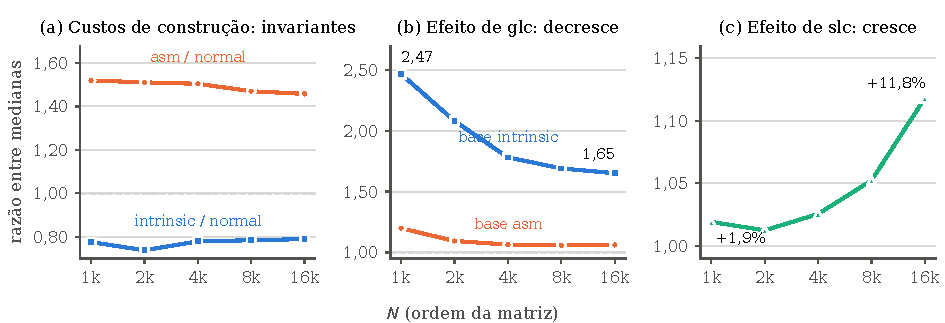
\includegraphics[width=\textwidth]{fig_sensibilidade}
\caption{Razões entre as medianas de dois cenários da Tabela~\ref{tab:sens}, no
mesmo $N$; numerador e denominador de cada curva estão na legenda. Acima de
1,00$\times$, o cenário do numerador é mais lento.}
\label{fig:sens}
\end{figure}

A Figura~\ref{fig:sens} separa fatores que se comportam de maneiras
qualitativamente distintas, e essa separação é o resultado central do
experimento. Os \textbf{custos de construção são estáveis} (curva~a): a barreira
de otimização imposta pelo bloco de \textit{assembly} custa entre 1,52$\times$ e
1,46$\times$ em toda a faixa, variação inferior a 5\% ao longo de um fator de
256 em volume de dados. É essa invariância que
permite descontá-los com segurança: são propriedades da geração de código, não
do comportamento de memória.

O \textbf{custo da \textit{flag} \texttt{glc}, ao contrário, não é estável}
(curva~b): medido sobre a base em \textit{assembly}, que mantém a construção
constante nos dois lados, cai de 1,20$\times$ em $N=1024$ para 1,06$\times$ em
$N=16384$. Em $N=1024$, campanhas independentes do mesmo \textit{kernel} deram
1,237$\times$ (Experimento~1) e 1,19$\times$ (Seção~\ref{sec:localidade}); a
queda com o tamanho excede essa variação. O contraste entre as curvas~a e~b é, em si,
evidência de que a \textit{flag} atua sobre o \textit{cache}: um custo de geração
de código não teria motivo para variar com o tamanho do problema, e de fato não
varia; o custo da \textit{flag} varia. O argumento é de contraste e não depende de
saber \emph{por que} varia. Cabe a ressalva de que este experimento estabelece a
dependência, mas não o mecanismo que a produz: com todos os tamanhos medidos
potências de dois, o crescimento do conjunto de trabalho e o agravamento das
condições de \textit{conflict miss} avançam juntos, e separá-los exige uma
varredura cruzando magnitude e alinhamento, apontada na Seção~\ref{sec:conclusao}
como o passo seguinte. Segue daí
que \textbf{uma medida em um único tamanho não caracteriza o efeito do
\textit{cache}}, e que reportá-la sem declarar o tamanho e a linha de base a
torna ininterpretável (Seção~\ref{sec:fatorial}).

\subsubsection*{O efeito de \texttt{slc} emerge apenas em conjuntos grandes}

O resultado mais informativo da análise está na curva~c da Figura~\ref{fig:sens}.
A \textit{flag} custa 1,9\% em $N=1024$, pouco, mas já acima do piso de ruído
da bancada. O efeito fica entre 1,2\% e 2,6\% até $N=4096$, cresce a partir daí e
alcança \textbf{11,8\% em $N=16384$}, duas ordens de grandeza acima do piso
daquele ponto.

Esse é exatamente o comportamento previsto para uma \textbf{política de
substituição}, e não para um \textit{bypass}. Marcar uma linha como candidata
preferencial a \textit{eviction} não produz efeito quando o conjunto de trabalho
cabe no \textit{cache}, pois não há disputa por espaço; o efeito só se manifesta
quando há mais dados concorrendo do que capacidade disponível: em $N=16384$,
três matrizes somando 3~GB contra 2~MB de L2. Um \textit{bypass} produziria
penalidade grande e aproximadamente constante, presente já nos tamanhos
pequenos. A análise corrobora, portanto, sob carga real e por via
independente, a conclusão obtida por vazão na Seção~\ref{sec:slc}.

\subsection{Experimento 4: Localidade do Padrão de Acesso}
\label{sec:localidade}

Os 45 pontos (três padrões, três configurações de \textit{flag} e cinco
tamanhos) foram validados sem divergência, com coeficiente de variação entre
0,02\% e 4,1\% em \textbf{linha} e \textbf{coluna} e de até 19,4\% em \textbf{dispersa}.

\begin{table}[ht]
\centering
\caption{Custo de contornar o L1 por padrão de acesso: razão entre a mediana com
a \textit{flag} e a mediana sem \textit{flag}, com a construção mantida constante.}
\label{tab:localidade}
\small
\begin{tabular}{@{}lrrrrr@{}}
\toprule
\textbf{Padrão} & \textbf{1024} & \textbf{2048} & \textbf{4096} & \textbf{8192} &
\textbf{16384} \\
\midrule
\multicolumn{6}{@{}l}{\textit{\texttt{glc}: desvio do L1}}\\
\tabinput{tab_loc_glc}
\midrule
\multicolumn{6}{@{}l}{\textit{\texttt{glc slc}: L1 e política do L2}}\\
\tabinput{tab_loc_glcslc}
\bottomrule
\end{tabular}
\end{table}

\textbf{O padrão \textbf{coluna} é quase indiferente ao L1.} Contorná-lo custa
entre 0,6\% e 1,4\%, com $cv$ entre 0,06\% e 2,5\%, efeito
pequeno, mas mensurável. Com passo de $4N$~bytes, cada iteração toca uma linha
nova, sem reúso dentro do \textit{work-item}, e removê-lo quase não custa. Nos padrões contíguos o mesmo desvio custa de 46\% a
119\%.

\textbf{O fator determinante é o reúso dentro da linha, não o \textit{broadcast}.}
Se o ganho do padrão \textbf{linha} viesse de 16 \textit{lanes} compartilharem
cada endereço, o padrão \textbf{dispersa}, que reduz esse compartilhamento a
até 4 e preserva o passo, deveria aproximar-se de \textbf{coluna}. Ele faz o oposto:
fica \emph{acima} de \textbf{linha} em todos os tamanhos. O que \textbf{linha} e
\textbf{dispersa} têm em comum, e \textbf{coluna} não tem, são os 16 acessos que
compartilham cada busca de 64~bytes. É esse reúso que confere valor ao L1.

\textbf{A penalidade do acesso disperso é dupla.} Antes de qualquer \textit{flag},
\textbf{dispersa} sustenta apenas 170--189~GB/s contra 783--798~GB/s de
\textbf{linha}, por tocar 19 linhas de \textit{cache} por instrução de
\textit{wavefront} em vez de 4. É o padrão mais caro em termos absolutos \emph{e} o que mais perde ao
ficar sem o L1.

\textbf{O \texttt{slc} confirma-se como política de evicção.} A metade inferior da
Tabela~\ref{tab:localidade} mostra seu efeito crescendo com a pressão sobre o L2:
desprezível em \textbf{coluna} nos tamanhos menores, chega a 1,233$\times$ em
$N=16384$; em \textbf{dispersa}, que mantém 19 linhas vivas por instrução,
alcança 3,376$\times$ em $N=8192$ e recua para 2,111$\times$ em $N=16384$, a única
queda expressiva do conjunto. Duas remedições independentes desses dois pontos
reproduzem o custo do \texttt{glc} a menos de 2,5\%, mas não o do \texttt{glc slc}
(3,016$\times$ e 3,360$\times$ em $N=8192$; 2,500$\times$ e 2,515$\times$ em
$N=16384$): a queda persiste nas três campanhas, de 17\% a 37\%, e a amplitude
entre elas, de até 12\% em $N=8192$ e 19\% em $N=16384$, supera a dispersão
interna, de até 7,4\%. As medianas das três campanhas são 3,360$\times$ e
2,500$\times$. Esses valores devem ser lidos com essa incerteza, e a queda não se
explica por saturação da política: com $B$ transposta (Tabela~\ref{tab:layout}),
no mesmo padrão de acesso, o efeito do \texttt{slc} continua crescendo em
$N=16384$.

\begin{table}[ht]
\centering
\caption{Multiplicação com $B$ usual e transposta: razões entre medianas. A
prevista soma os padrões isolados da Tabela~\ref{tab:localidade}
(\textbf{linha}+\textbf{dispersa} sobre \textbf{linha}+\textbf{coluna}).}
\label{tab:layout}
\small
\begin{tabular}{@{}lrrrrr@{}}
\toprule
 & \textbf{1024} & \textbf{2048} & \textbf{4096} & \textbf{8192} & \textbf{16384} \\
\midrule
\tabinput{tab_layout}
\bottomrule
\end{tabular}
\end{table}

\textbf{A conclusão se transfere para o algoritmo completo.} Nos 30 pontos da
Tabela~\ref{tab:layout}, todos validados, transpor $B$ torna a multiplicação \textbf{2,31 a 2,46$\times$ mais
lenta} sem \textit{flag} alguma (203--207 contra 82--89~GFLOPS), de modo
estável nos cinco tamanhos. Ganha-se contiguidade dentro de cada \textit{lane} e
perde-se a coalescência entre \textit{lanes}: o acesso a $B$ passa de
\textbf{coluna} a \textbf{dispersa}, e a soma dos padrões isolados prevê a razão
com erro abaixo de 3\% a partir de $N=2048$ (8\% em $N=1024$). A previsão vale só
com os \textit{caches} ligados; sob \texttt{glc} subestima a razão em até 16\%. A
lição é de alinhamento, não de transposição: na GPU o eixo decisivo é o que varia
entre \textit{lanes}, e o \textit{layout} usual já é o favorável ao mapeamento
adotado. O resultado vale para o \textit{kernel} sem \textit{tiling}.

\textbf{A dependência do L1 acompanha o padrão.} Com $B$ transposta, contornar o L1
custa de 1,96 a 1,48$\times$, contra 1,19 a 1,05$\times$ no \textit{layout} usual.
Esta última série é o mesmo \textit{kernel} do Experimento~3, medido em campanha
independente, e reproduz a curva~b da Figura~\ref{fig:sens} com diferença
máxima de 2,1 pontos percentuais.

\section{Conclusões e Trabalhos Futuros}
\label{sec:conclusao}

Este trabalho mediu o impacto da hierarquia de memória no desempenho de uma GPU
AMD Polaris (gfx803) sob OpenCL, usando como instrumento o controle explícito das
\textit{flags} de \textit{cache}. Os quatro experimentos permitem três conclusões.

A primeira, e central, é que \textbf{o valor do L1 não é uma constante da
arquitetura, e sim função do problema e do padrão de acesso}. Ao longo de um fator
de 256 em volume de dados, o custo de contorná-lo cai de 1,20$\times$ para
1,06$\times$, enquanto o custo de construção permanece invariante, evidência de
que a \textit{flag} atua sobre o \textit{cache} (Seção~\ref{sec:sens}). E varia mais ainda com a localidade: mantidos a matriz, o número de
\textit{loads} e a construção, contornar o L1 custa até 2,19$\times$ num percurso
contíguo e 1,01$\times$ num percurso por coluna, praticamente nulo. O fator
determinante não é o compartilhamento de endereço entre \textit{lanes},
cuja redução \emph{aumenta} a dependência do \textit{cache}, e sim o reúso dentro
da linha de 64~bytes. A conclusão se transfere para o algoritmo completo: transpor
$B$, otimização clássica em CPU, torna a multiplicação 2,3 a 2,5$\times$ mais lenta,
razão que a soma dos padrões isolados prevê.

A segunda é que, \textbf{em leituras FLAT, apenas um limite da hierarquia é
selecionável por \textit{flags} de instrução}. A \textit{flag} \texttt{glc}
contorna o L1 de forma verificável na ISA e mensurável em desempenho; \texttt{slc}
não produz \textit{bypass} do L2, e a refutação vem por três vias: um conjunto
que cabe no L2 sustenta 555,9~GB/s, acima do pico teórico de 256~GB/s que limita
qualquer leitura atendida pela VRAM; logo acima da capacidade do L2, a
\textit{flag} \emph{acelera} a leitura em até 1,51$\times$, retendo parte do
conjunto; e, na multiplicação, seu custo cresce com o conjunto de trabalho. As
duas últimas são assinaturas de política de \textit{eviction}. Por esse meio não há caminho direto à VRAM,
embora o manual descreva o SLC, nos formatos MUBUF e MTBUF, como forçando a falta
no L2.

A terceira é metodológica: \textbf{a comparação ingênua superestima o efeito do
\textit{cache}}. O mecanismo mais acessível, o \texttt{volatile}, emite a
\textit{flag} sob o Clang/LLVM e não sob o compilador proprietário e, onde a emite,
serializa os \textit{loads}; o bloco de \textit{inline assembly} custa por si só
cerca de 1,5$\times$. Isolá-los exigiu cenários de controle sem \textit{flag}
alguma e um par de \textit{kernels} de fonte idêntico, que funciona como controle
negativo e fixa em 0,14\% o menor efeito afirmado. A referência em CPU tornou
visível, por fim, que a vantagem da GPU sobre o mesmo algoritmo cresce de
35$\times$ para 400$\times$ com o tamanho: também aí é a hierarquia de memória, e
não a capacidade aritmética, que governa a diferença.

Frente à literatura, os resultados complementam os estudos de
\textit{microbenchmarking} em GPUs NVIDIA~\cite{wong2010, mei2017, jia2018}, que
caracterizam latência e capacidade de cada nível, ao medir quanto um nível vale
para um algoritmo e do que esse valor depende, numa arquitetura AMD sob OpenCL que
aqueles trabalhos não cobrem. Diante de Jia, Shaw e Martonosi~\cite{jia2012}, que
fizeram a pergunta no Fermi, concordam em que o L1 não aproveita o
compartilhamento de endereço entre \textit{lanes} e divergem em dois pontos: lá o
L1 não aproveitou, no caso testado, o reúso entre instruções da mesma
\textit{thread}, aqui sua principal fonte de valor; e lá chegou a retardar
programas, enquanto aqui contorná-lo nunca acelerou. Confirmam também que o acesso
à memória domina o
desempenho~\cite{seo2011} e quantificam o peso da organização dos
\textit{work-items}~\cite{fraire2013}, que decide o custo da transposição. E
qualificam a atribuição ao sistema operacional das diferenças entre
plataformas~\cite{vidye2023, balen2022}: sobre o mesmo dispositivo, a diferença
decorreu do compilador, em linha com o que Fang et al.~\cite{fang2011} observaram
no código gerado para OpenCL.

Como limitações, os resultados provêm de uma única geração de \textit{hardware};
apenas leituras FLAT sobre a VRAM foram investigadas, ficando em aberto o
comportamento das \textit{flags} em escrita, no formato MUBUF e em outros tipos de
memória (MTYPE); e todos os tamanhos medidos são potências de dois, de
modo que o crescimento do conjunto de trabalho e o agravamento das condições de
\textit{conflict miss} avançam juntos. Como trabalhos futuros, propõe-se um
desenho fatorial cruzando magnitude e alinhamento, capaz de separar os dois
efeitos e de estabelecer o mecanismo que este trabalho apenas constata, e a
caracterização por latência, com \textit{pointer chasing} sob controle de
\textit{flags}.

\section*{Declaração de uso de ferramentas de Inteligência Artificial}

Utilizou-se o Claude Code (Anthropic), com os modelos Claude Opus~5 e Claude
Opus~5.5, como apoio ao planejamento, à implementação e à execução dos
experimentos, bem como à redação e à revisão de todas as seções do texto.

\bibliographystyle{sbc}
\bibliography{sbc-template}

\end{document}
